\documentclass[]{scrartcl}
\usepackage{Preamble}

\setcounter{section}{5}
\newcommand{\exercise}{Exercise \thesection}
\newcommand{\duedate}{2020-12-21, 23:59}

\begin{document}
\section*{\exercise}

To compile: unzip our uploaded code, and run \verb|make| inside \verb|code/|.
The slurm scripts are stored inside \verb|code/slurm/|.

To debug: run the debug outputs (\verb|*.dbg|) and attach gdb to respective pids

\subsection{Reading}
\subsection{Heat Relaxation --- Sequential Implementation}\label{ssec:heat_seq}
(see \verb|code/|)
Visualization in \href{./img/heat.gif}{img/heat.gif}
\subsection{Heat Relaxation --- Experiments}
The Sequential Heat Relaxation Implementation of \autoref{ssec:heat_seq} resulted in the values observed in \autoref{tab:heat}.
These Numbers resulted from 100 iterations per grid size, with two buffers.
\begin{table}[ht]
    \centering
    \caption{Resulting Numbers for a sequential Heat Relaxation}\label{tab:heat}
    \begin{tabular}{lrrr}
\toprule
{} &    NP = 1 &   NP = 2 &   NP = 4 \\
Grid size &           &          &          \\
\midrule
100x100   & 1000.0000 &      NaN &   7.7300 \\
200x200   & 1000.0000 &      NaN &  27.8900 \\
300x300   & 1000.0000 &      NaN &  67.1000 \\
400x400   & 1000.0000 &      NaN & 134.2000 \\
500x500   & 1000.0000 & 200.0000 & 135.0400 \\
\bottomrule
\end{tabular}

\end{table}

\begin{figure}[H]
    \centering
    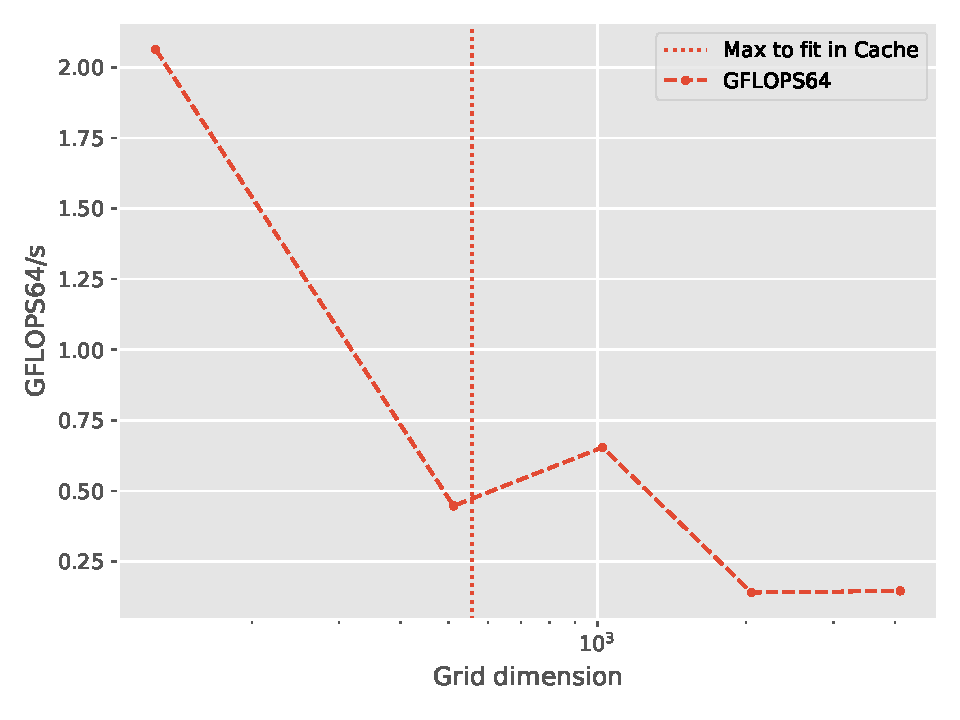
\includegraphics[]{img/heat.pdf}
    \caption{Resulting GFLOPS64 for increasing Dimensions, with the maximum dimension for fitting both buffers into cache marked}\label{fig:heat}
\end{figure}

The resulting numbers are not surprising.
The Size Limit for fitting both buffers into Cache\footnote{10MB for a Intel Xeon E5-1620}, when reached will result in the effective GFLOPS plummeting.


\begin{align}
    \text{Max Grid Size} &= \sqrt{\frac{\text{Cache Size}}{\text{Byte per Double} \cdot \text{\# of Buffers}}}\\
                                  &= \sqrt{\frac{\SI{10}{MB}}{\SI{8}{B}\cdot 2}}\\
                                  &\approx 790
\end{align}

But these Numbers represent the maximum possible dimension if nothing else has to be stored in the cache.

When increasing the dimension further, a further decrease in performance will be expected, due to an increase in cache misses.

\subsection{Heat Relaxation --- Pre-considerations for parallelization}
Some considerations for applying MPI to the heat relaxation problem:

\begin{enumerate}
    \item To de-compose the complete problem into subtasks would mean splitting the grid into parts for which a separate rank is responsible.
        This would require the ability to communicate between ``neighboring'' ranks.
    \item For this grid either 1D or 2D partitioning is possible, e.g.: splitting the MxN Grid into 4 rectangles with one dimension equal to the original grid ($\frac M4$xN or Mx$\frac N4$) or splitting the complete Grid into 4 rectangles of the same aspect ratio as the original ($\frac M2$x$\frac N2$).

    The better partitioning for a given Problem would be the one, in which we are required to exchange fewer grid points (Volume-Surface Rule).
    \autoref{fig:partitioning} demonstrates this rule: here all fully filled grid-points are calculated by a corresponding rank.
    The not filled outlines represent the points required by the same colored rank for its next iteration, which are calculated by a neighbor.
    When these surfaces are calculated they are exchanged with the corresponding neighbor.

    \begin{figure}[H]
        \centering
        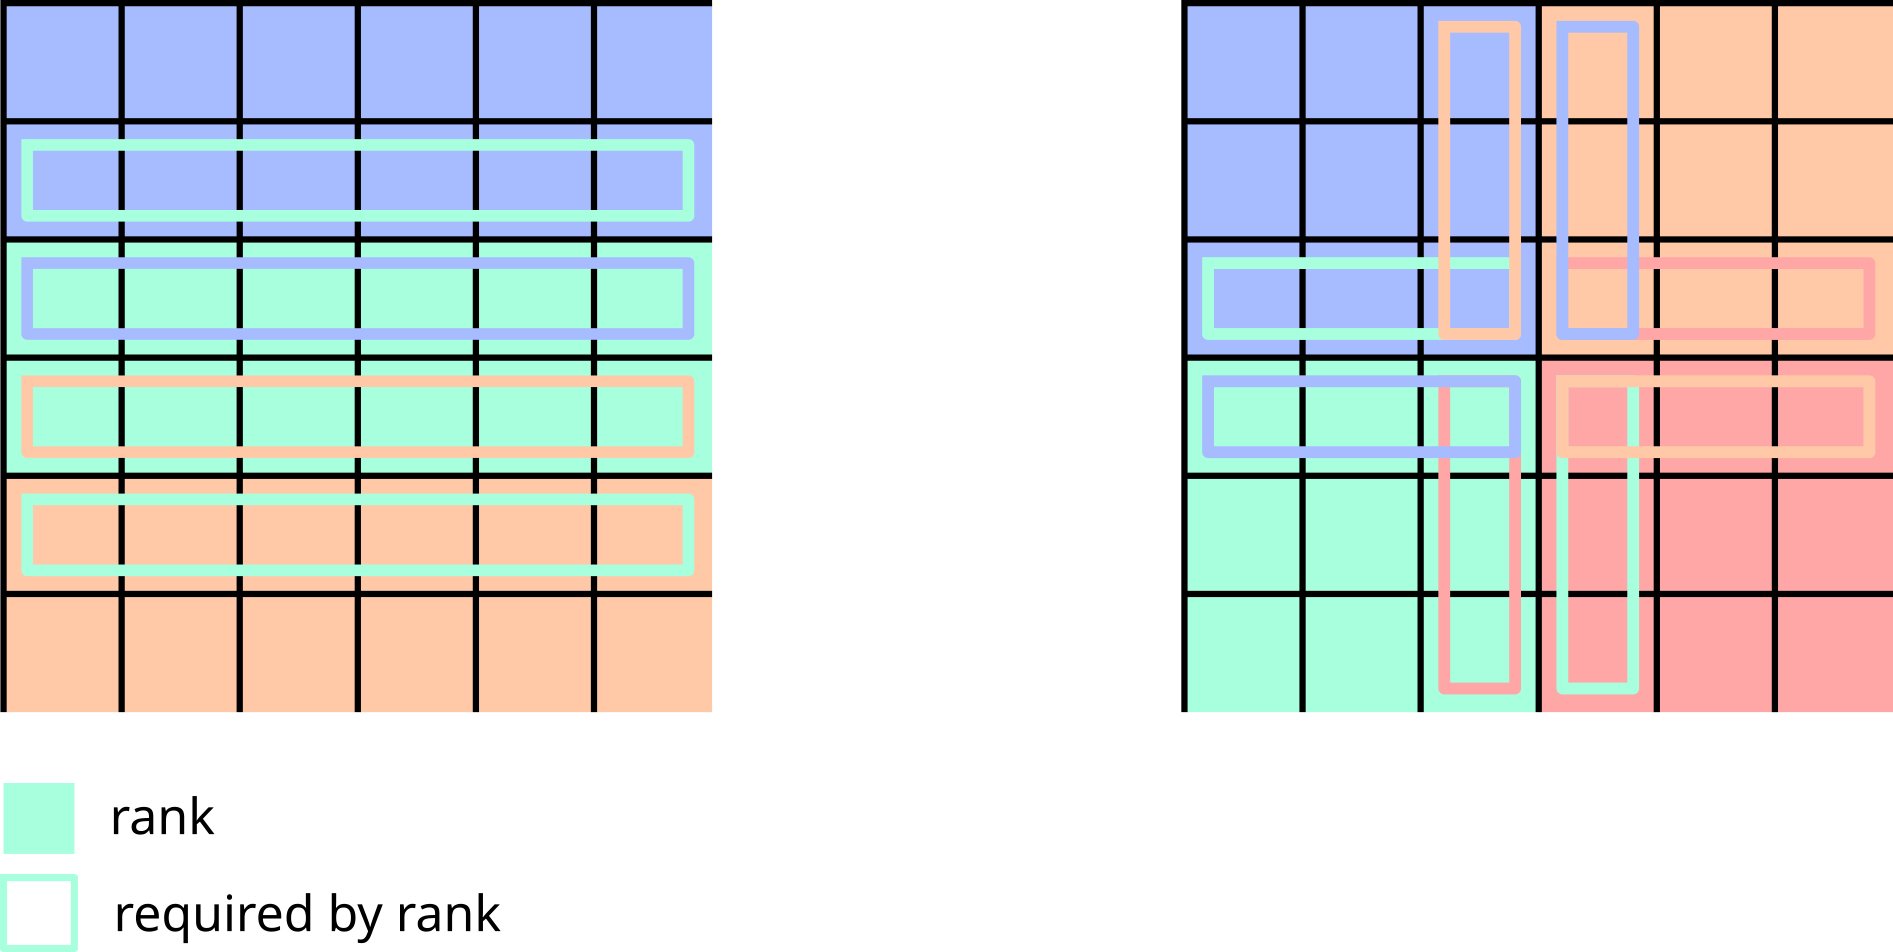
\includegraphics[width=0.8\linewidth]{img/partitioning.png}
        \caption{Example of Partitioning Schemes, 1D (NS) on the left, 2D (NEWS) on the right}%
        \label{fig:partitioning}
    \end{figure}

    With the Example of before (4 ranks, MxN Grid, 1D (North-South) and 2D (NEWS) Partitioning), we would need to exchange the following number of points for each method:

    \begin{align}
        \text{\# exchanged points}_\text{1D, NS} &= N \cdot 2 \cdot \text{\# partitions} - \text{\# border partitions}\\
                                                    &= N\cdot 2 \cdot 4 - 2 = \mathbf{8N-2}
    \end{align}
    \begin{align}
        \text{\# exchanged points}_\text{2D, NEWS} &= \sqrt{\text{\# partitions}} \cdot 2 \cdot N \nonumber\\
                                                      &+ \sqrt{\text{\# partitions}} \cdot 2 \cdot M - \text{\# border partitions}\\
                                                      &= \mathbf{4N + 4M - 4}
    \end{align}

    {\bfseries That means for our use case (big and nearly square grids) the 2D partitioning will always require less points to be exchanged.}

    \item We know that only the points near the surfaces need to be exchanged.
        To minimize delays due to these calculations, we should calculate the surface points ideally the moment their required neighbors are available and send them off immediately.
        This is allowing the rest of the volume to be calculated in the meantime.

    \begin{figure}[H]
        \centering
        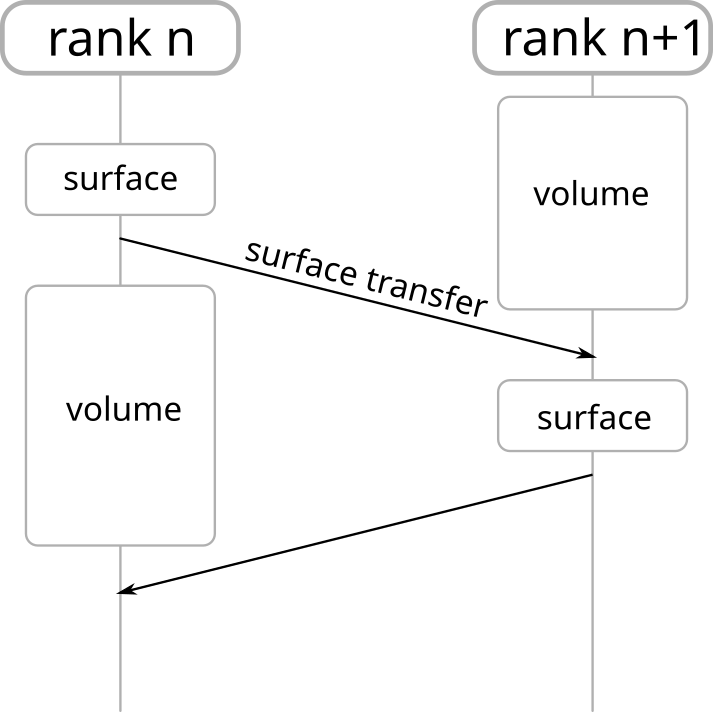
\includegraphics[width=.4\linewidth]{img/transfer.png}
        \caption{Transfer and Priority of Surface Calculations}%
        \label{fig:transfer}
    \end{figure}
\end{enumerate}

\end{document}
